

\begin{figure}[ht]
\centering
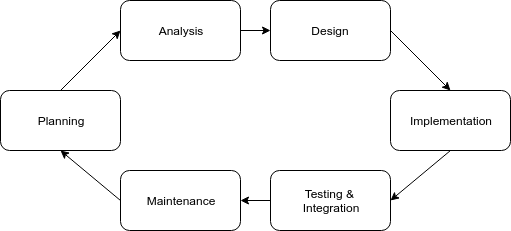
\includegraphics[width=.6\linewidth]{resource/img/ch_intro/sdlc.png}
\caption{Software Development Life Cycle}
\label{fig:intro:sdlc_redo}
\end{figure} 

% \begin{figure}[ht]
% \centering
% 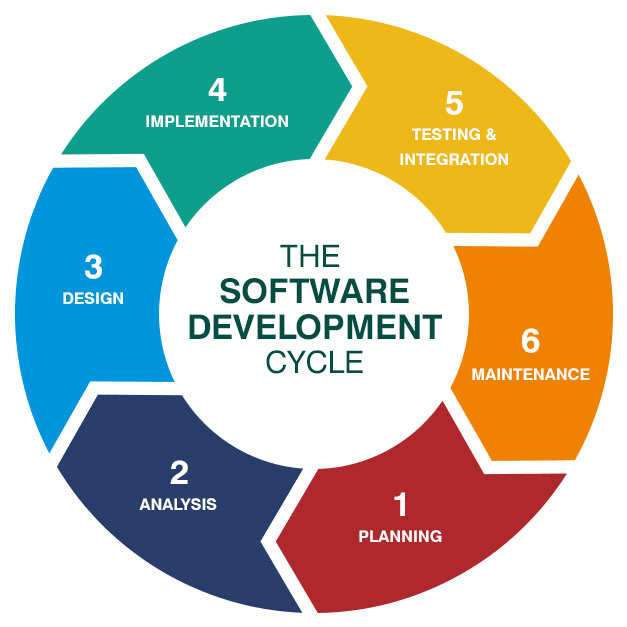
\includegraphics[width=.6\linewidth]{resource/img/ch_intro/sdlc_from_google.png}
% \caption{Software Development Life Cycle}
% \label{fig:intro:sdlc_redo}
% \end{figure} 

The software development life cycle shown in Figure \ref{fig:intro:sdlc_redo} is an iterative process that, until recently, was almost exclusively used within the Software \& Platform KA. Before the Agile\cite{Beck_2013} method was adopted, a single iteration of the SDLC could span several years, with planning, design, and analysis consuming a significant portion of the up front time and cost for the project. When a software project failed under this model, it happened because available funding was burned and often resulted in little or no working code. The Agile approach prefers faster iterations (often counted in weeks) with less emphasis on up front specifications. The result is a 'fail-fast' model that surfaces fundamental problems early and produces prototype software that may be salvaged and reused in other work if the project is abandoned. 

An ecosystem of tools exists around the SDLC that are mature, actively maintained, and most importantly (for us at least) almost entirely automated. Design requirements are captured in trackers that contain customizable metadata like priority, status, and dependencies. These requirements can link to code commits or PRs that satisfy the requirement, or customer created issues or development blockers that prevent the requirement from being closed. Unit, Integration, Regression, and Acceptance tests are run by continuous integration and delivery systems which can prevent breaking changes from entering the code base, roll back bad commits that do get merged, and deploy updates to production servers as dictated by the pipeline configuration. 

As an extension (and tacit endorsement) of the automated software CI/CD pipeline described above, development operations(DevOps) has recently emerged as the corollary in managing the life cycles components in the System and Infrastructure CyBOK categories. DevOps allows systems and network engineers to develop, test, deploy, and provision the supporting infrastructure required by an application in the same workflow, even from the same code base as the desired application. Maintaining the desired state of the underlying system in configuration files and provisioning scripts through a version control system is often called \textit{Infrastructure-as-Code}, While this is sometimes used to set up bare metal resources like servers and network appliances, the more common case currently is to provision infrastructure onto a self managed or commercial hypervisor using virtual machines or containerized micro services. 

\begin{figure}[ht]
\centering
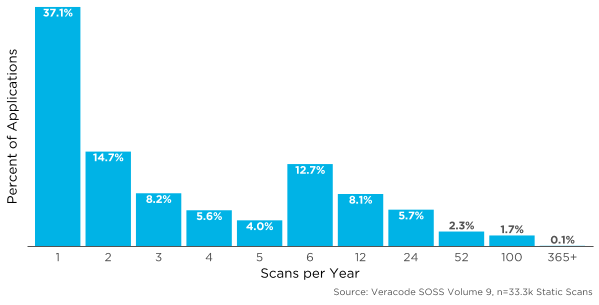
\includegraphics[width=.9\linewidth]{resource/img/ch_intro/veracode_scanfreq_percentages.png}
\caption{Veracode Freq Percentages SOSS \cite{soss_v9}}
\label{fig:intro:soss-scan-freq}
\end{figure} 

A functioning DevOps workflow integrates the application development and operations teams. The next logical step in this evolution is to disentangle the stovepiped security evaluation mechanisms built around each of these formerly independent areas. The resulting field of SecDevOps (or DevSecOps\cite{Rahman_Williams_2016}) is \textit{not} the sum of the security of each part (although it will likely be treated that way at least until the community converges on which term to reference it by). Rather, it should trigger a re-assessment of previous security controls and best practices prescribed through existing regulatory and compliance frameworks. 

For example, Figure \ref{fig:intro:soss-scan-freq} shows the yearly count from over 33 thousand source code scans in 2018 as reported by Veracode. While this data is from a single vendor, the results are still concerning. The median number of security scans per year was just 2. We presume there is regulatory or compliance pressure to scan at least once per year. Given the percentage of applications that scan once a week or more is just over 4\%, we can also infer that most customers either don't have an automated development workflow in house, or if they do have chosen not to integrate this capability. 


\begin{figure}[ht]
\centering
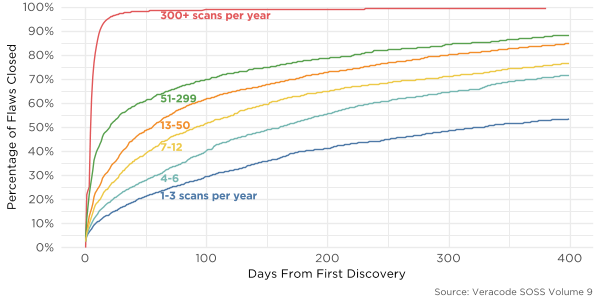
\includegraphics[width=.9\linewidth]{resource/img/ch_intro/veracode_scanfreq_vs_closures.png}
\caption{Veracode Scan Frequencies vs Closures SOSS \cite{soss_v9}}
\label{fig:intro:soss-scan-freq-closures}
\end{figure} 

While we can't extrapolate with confidence the closure rates in Figure \ref{fig:intro:soss-survival} to CVSS findings, or the scan rates in Figure \ref{fig:intro:soss-scan-freq} to users of alternative static analysis products, we can draw a very clear line between the teams that scan their code as part of an automated development workflow and their ability to address security findings. Figure \ref{fig:intro:soss-scan-freq-closures} displays a distinct stratification of response times based on scan frequency. Indeed, the teams that incorporated a simple static analysis check into their DevOps pipeline were able to remediate nearly all found flaws before the others could fix half. What we observed from Figure \ref{fig:intro:soss-survival}, that around half the observed samples only conducted one or two scans per year suggests that, in this context, they were only able to fix about 50\% of the identified flaws after more than 400 days. Referring back to the Agile development principals that DevOps workflows are based upon, we can surmise the relative speed in addressing flaws is attributable to small incremental changes with actionable feedback after each change. 




% The motivation of this thesis is to make modern information systems more secure, and the driving force behind that goal is automation. Many of the problems addressed in this work stem from the disparate ecosystem of tools, APIs, methodologies, libraries, and frameworks that exist in relative isolation to one another. 

% Consider Security Information and Event Management (SIEM) systems as an example, which provide correlation of host/network event logs, IDS/IPS alerts, threat/vulnerability feeds, etc, and present a unified view of the system’s security posture automatically to the SOC. Before the advent of managed SIEMs, sys admins typically filled the role of security engineers, and relied on hand rolled collections of shell/perl scripts to manage systems, parse logs, collect or push events, format reports, and issue alarms. To be effective required tribal knowledge along with proficiency in programming, network plumbing, and systems management, so changes to the environment or workforce made it extremely difficult(expensive) to deliver continuous monitoring capabilities to operators at any scale. 
% We are in a similar state today with network design and enterprise planning. Infrastructure-as-Code, SDN, virtualization and containerization are all critical components in modern deployments, but the glue that ties them together is largely ad-hoc, and risk evaluation is still a manual task. 




% In order to understand the security posture before a system is rolled out and SIEMs are in place, we are creating a tool to facilitate the automated analysis, collection, correlation, and dissemination of the security metrics mentioned above. The necessity of such a tool is critical to evaluating the efficacy of the metrics reviewed above, and provides the foundation for ongoing research in machine learning models for secure systems planning, design, and evolution.




% \textbf{Software Security Metrics} 

